\documentclass[12pt]{article}

\usepackage[letterpaper,margin=0.7in]{geometry}
\usepackage[T1]{fontenc}
\usepackage{newtxtext}
\usepackage{lipsum}

% Figure stuff
\usepackage{floatrow}
\usepackage{multirow}
\usepackage{booktabs}
\setlength{\heavyrulewidth}{1.5pt}
\setlength{\abovetopsep}{4pt}

\usepackage{enumitem}
\setlist[enumerate]{itemsep=0mm}
%\usepackage{paralist}


% ToC
\usepackage{blindtext} 
\usepackage[linktocpage]{hyperref}
\usepackage{bookmark}
\usepackage[compact]{titlesec}

% bib
%\usepackage[round]{natbib}
\usepackage[square,sort,numbers]{natbib}

% Math Imports
\usepackage{amsmath, amssymb, bm, fancyhdr, sectsty, dsfont, mathtools}

% Tikz
\usepackage{tikz}
\usetikzlibrary{bayesnet}
\usetikzlibrary{arrows}
\usepackage{tikz}
\usepackage{tikz-dependency}
\usetikzlibrary{shapes.arrows, positioning, fit, bayesnet,
    arrows,backgrounds,patterns,matrix,calc,shadows,plotmarks,
    shapes,positioning,automata,positioning,spy,scopes,chains,decorations,decorations.pathreplacing}
\pgfdeclarelayer{background}
\pgfdeclarelayer{foreground}
\pgfsetlayers{background,main,foreground}

\usepackage{wrapfig}
\usepackage{comment}
\usepackage{subcaption}
\usepackage{cleveref}

\usepackage[font=small]{caption}

% Symbols
\newcommand\ind{\protect\mathpalette{\protect\independenT}{\perp}}
\def\independenT#1#2{\mathrel{\rlap{$#1#2$}\mkern2mu{#1#2}}}
\newcommand\norm[1]{\left\lVert#1\right\rVert}
\newcommand\set[1]{\left\{#1\right\}}

\newcommand\RNN{\mathrm{RNN}}
\newcommand\MLP{\mathrm{MLP}}
\newcommand\enc{\mathrm{enc}}
\newcommand\softmax{\mathrm{softmax}}

% Distributions
\newcommand{\Cat}{\mathrm{Cat}}
\newcommand\Expo{\mathrm{Expo}}
\newcommand\Bern{\mathrm{Bern}}
\newcommand\Pois{\mathrm{Pois}}
\newcommand\Bin{\mathrm{Bin}}
\newcommand\Unif{\mathrm{Unif}}
\newcommand\Betad{\mathrm{Beta}}
\newcommand\Gammad{\mathrm{Gamma}}
\newcommand\Geom{\mathrm{Geom}}
\newcommand\Logd{\mathrm{Logistic}}

\newcommand\E[1]{\mathbb{E}\left[#1\right]}
\newcommand\Es[2]{\mathbb{E}_{#1}\left[#2\right]}
\newcommand{\Var}{\mathrm{Var}}
\newcommand{\Cov}{\mathrm{Cov}}
\newcommand{\Cor}{\mathrm{Cor}}

% Bold stuff
\newcommand{\ba}{\mathbf{a}}
\newcommand{\bb}{\mathbf{b}}
\newcommand{\bc}{\mathbf{c}}
\newcommand{\bd}{\mathbf{d}}
\newcommand{\be}{\mathbf{e}}
\newcommand{\bg}{\mathbf{g}}
\newcommand{\bh}{\mathbf{h}}
\newcommand{\br}{\mathbf{r}}
\newcommand{\bs}{\mathbf{s}}
\newcommand{\bt}{\mathbf{t}}
\newcommand{\bv}{\mathbf{v}}
\newcommand{\bw}{\mathbf{w}}
\newcommand{\bx}{\mathbf{x}}
\newcommand{\by}{\mathbf{y}}
\newcommand{\bz}{\mathbf{z}}

% mathcal stuff
\newcommand{\mcD}{\mathcal{D}}

% math blackboard bold stuff
\newcommand{\R}{\mathbb{R}}
\newcommand{\C}{\mathbb{C}}
\newcommand{\Z}{\mathbb{Z}}
\newcommand{\N}{\mathbb{N}}
\newcommand{\Q}{\mathbb{Q}}


\DeclareMathOperator*{\argmin}{argmin}
\DeclareMathOperator*{\argmax}{argmax}

\titlespacing{\paragraph}{0pt}{*0}{*0}
%\setlength{\parskip}{-5mm plus1mm minus1mm}

\makeatletter
\newcommand{\subalign}[1]{%
  \vcenter{%
    \Let@ \restore@math@cr \default@tag
    \baselineskip\fontdimen10 \scriptfont\tw@
    \advance\baselineskip\fontdimen12 \scriptfont\tw@
    \lineskip\thr@@\fontdimen8 \scriptfont\thr@@
    \lineskiplimit\lineskip
    \ialign{\hfil$\m@th\scriptstyle##$&$\m@th\scriptstyle{}##$\crcr
      #1\crcr
    }%
  }
}
\makeatother

\usepackage{fancyhdr}
\pagestyle{fancy}

\usepackage[displaymath,mathlines]{lineno}
\linenumbers

\begin{document}
\lhead{Justin Chiu}
\chead{2018 NDSEG Application}
\rhead{Research Proposal}

\begin{center}
%\textbf{Exploiting the Duality of Natural Language Generation and Understanding}
\textbf{Information Extraction with Distant Supervision}
\end{center}

\paragraph{Keywords}
information networks, natural language processing, information extraction, latent variable models

\paragraph{Relevance to Army BAA: II. A. c. iii. (3) Information Networks}
% Introduce knowledge graphs
In order to provide decision makers with the information
necessary to make informed choices as well as predict the effects of those choices,
we must have an efficient representation of relevant information and a predictive model
for the resultant state of the world after a choice is made.
Information networks provide a graphical representation of information and how it
propagates through a network.
I focus on \textit{knowledge graphs}, information networks where each node contains a set of facts
about an entity and an edge describes how the facts in one node influence the facts in another.
% We allow self-loops
Knowledge graphs provide an intuitive and queryable representation of knowledge.
A decision maker may query the relevant nodes to gain situational awareness, and
when simulating a decision that alters the information in one node
the graph can easily propagate those changes by virtue of its representation.

Given that a knowledge graph must represent an extremely large number of facts and relationships,
it is infeasible to specify these completely by hand.
I propose to fill in the nodes of a knowledge graph by leveraging a generative model
of corpora.
Many recent works have taken an orthogonal direction known as link prediction,
which fills in the missing \textit{edges} of a knowledge graph \citep{chen2018diva}.
Through link prediction one uses the relationships
specified by the edges to reason about the facts contained in a node conditioned on
the facts of its neighbours.
However, we generally also have access to large amounts of unlabeled and unstructured data
in the form of natural language corpora.
I aim to leverage natural language corpora by
learning an information extraction system that is able to 
extract facts from text to fill in the nodes of a knowledge graph
given only the assumption that the text was generated from the information
represented in the knowledge graph.

In this proposal I present a method towards automating the
training of information extraction systems with unlabeled corpora
by recasting the information extraction problem as a conditional generative modeling problem.
We propose to perform information extraction by first modeling the 
generative process of writing the text given the data,
then inverting that process in a probabilistically principled manner
through posterior inference.

\paragraph{Background}
% Information extraction
The goal of information extraction is to produce structured representations of information
given unstructured text.
Figure~\ref{fig:d2t} is an example of a datum and text pair which may be used to
train an information extraction system, inspired by the Rotowire dataset \citep{wiseman2017d2t}.
A typical approach to an information extraction system is the following pipeline:
\begin{enumerate}
\item First segment the text into mentions and values, i.e. michael jordan and all numerical values.
\item Then align the mentions to a entity, a node in a knowledge graph.
The node of interest is labelled `michael jordan'.
\item Finally identify the relationships between segments.
The relationships between these segments entail facts, which
are below the summary in Figure~\ref{fig:d2t}.
\end{enumerate}

Given the large cost of obtaining labels to train an extraction system,
a model that can perform well with less supervision is appealing.
For example, consider the case where Figure~\ref{fig:boxscore} is missing all values except for 
Michael Jordan's name.
In this scenario, where there is an availability of text but a lack of facts,
learning to write the text is much easier than training an extraction system
since the lack of facts results in a lack of labels for the extraction system.
A model that creates text as well as facts is called a generative model.
A generative model is defined by its generative process, which 
is a recipe for how the dataset is created.
A generative model that includes latent or unobserved variables in its generative process
is a latent variable model (LVM).
The benefit of using a LVM rather than directly modeling facts given text is two-fold:
\begin{enumerate}
\item An LVM can learn in the semi-supervised or unsupervised setting,
where only a few labels or no labels are provided respectively.
This implies we can train a model with missing facts.
\item LVMs provide a principled approach to inverting their generative process,
allowing one to reason about unobserved quantities earlier in the process given
observations later in the process. 
\end{enumerate}

\begin{figure}[t]
\centering
\floatbox[{\capbeside\thisfloatsetup{capbesideposition={left,top},capbesidewidth=4cm}}]{figure}[\FBwidth]
{\caption{A simplified example of a summary generated from a set of facts about an entity.
A full dataset consists of many unaligned sets of facts and sentences.}
\label{fig:boxscore}}
{\small\begin{tabular}{ccc|c}
\toprule
Entity & Type & Value & Summary\\
\midrule
michael jordan & NAME & michael jordan &
\multirow{4}{*}{\parbox{4cm}{michael jordan had 22 points and 12 rebounds as well as four blocks}}\\
michael jordan & POINTS & 22 &\\
michael jordan & REBOUNDS & 12 & \\
michael jordan & BLOCKS & 4 &\\
\bottomrule
\end{tabular}}
%\caption{An example of a set of facts from a basketball game paired with a statement generated from them.}
%\label{fig:boxscore}
\end{figure}

In this proposal, I focus on the class of LVMs known as hidden semi-Markov models (HSMMs),
used in \citet{liang2009semalign} as a conditional generative model for the
task of aligning segments of text to nodes in a knowledge graph without supervision.
\citet{liang2009semalign} rely on the insight that a conditional generative model of text
provides signal for learning the alignments:
if the likelihood of a segment of text improves when moving from
one alignment choice to a another,
then the new alignment is more likely to be correct given a suitably strong likelihood model.
The same intuition can be used to formulate a LVM for a semi-supervised information extraction system
which aims to model not just the alignments from segments of text to nodes in a knowledge graph
but also the values in the nodes themselves.
We build on the formulation in \citet{liang2009semalign} by parameterizing our LVM
with neural networks, drastically increasing the generative model's capacity.

\paragraph{Problem Setup}
We consider datasets consisting of aligned data and text
$\set{(\br^{(1)}, \by^{(1)}),(\br^{(2)},\by^{(2)})\ldots}$.
For brevity, I refer to a single datum and text as $\br,\by$, omitting the superscript.
Each datum $\br = \set{r_1,\ldots,r_N}$ is a set of $N$ records, where each record $r_i = (e_i, t_i, v_i)$
is a tuple containing an entity, type, and value.
The datum $\br$ is a knowledge base, or equivalently an information network
without a representation of the causal effects between records.
We refer collectively to all the entities, types, and values in a given datum $\br$ as
$\be,\bt,\bv$ respectively.
Each text $\by = \set{y_1,\ldots,y_T}$ is a sequence of tokens each from a vocabulary $V$.

The Rotowire dataset \citep{wiseman2017d2t} is an example of such a dataset.
Rotowire contains summaries of basketball games $\by$ aligned with the respective
box scores $\br$ of those games.
Consider the datum in Figure~\ref{fig:d2t} that consists of three records
and the statement $\by = $ ``michael jordan had 22 points and 12 rebounds as well as four blocks''.
For this example, the process of information extraction is to infer 
the values $\bv$ of the records given the entities $\be$, types $\bt$, and the text $\by$.

\paragraph{Proposal}
We propose to verify the efficacy of the LVM framework in the
semi-supervised information extraction setting,
with the following goals:
\begin{enumerate}
\item By formulating a LVM for generating text conditioned on data,
    obtain an information extraction system through posterior inference.
\item Demonstrate strong extractive performance with minimal labels.
\item Move towards a model for knowledge graph completion that captures
    the full joint distribution.
\end{enumerate}
We present one instance of a LVM and outline how it can be used to obtain
an information extraction model without direct supervision,
then argue that the same approach can be applied in even more ambitious settings.
Our proposed LVM is a conditional generative model that specifies
the relationship between data, specifically the entities and types, and text.
We denote this model \texttt{Values}.
%Let $\by$ be the text, $\ba$ be a latent variable that represents the
%alignments from words to records,
%$\bv$ all the values in a datum of records,
%and $\be,\bt$ the entities and types respectively.
Our model takes the form of a hidden semi-Markov model (HSMM),
where the model learns to generate the values, record alignments, and finally the text.
\begin{figure}[t]
\centering
\floatbox[{\capbeside\thisfloatsetup{capbesideposition={left,top},capbesidewidth=4cm}}]{figure}[\FBwidth]
{\caption{An example of our proposed information extraction procedure
with an inferred segmentation and values, which the model gathers evidence for
from the text. The values that must be inferred are in curly braces.}
\label{fig:d2t}}
{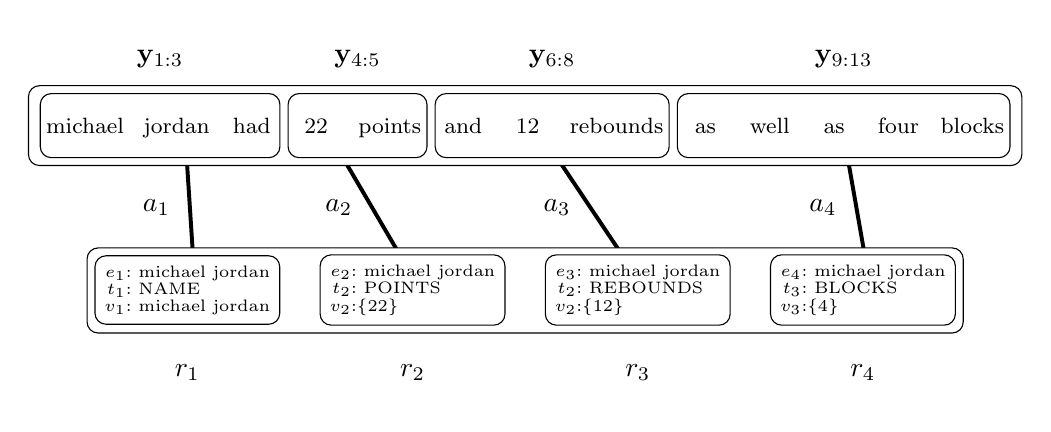
\begin{tikzpicture}[every node/.style={anchor=base,minimum size=8mm}]
\matrix (txt) [matrix of nodes, row sep=0.5em,column sep=0.05em,
    minimum width=0em, minimum height=1em, font=\footnotesize,ampersand replacement=\&,
    text height=.6em,text depth=.05em] {
      michael\& jordan \& % 1-2
      had \& % 3
      22\& points \& % 4-5
      and \& % 6
      12\& rebounds \& % 7-8
      as\& well\& as \& % 9-11
      four\& blocks % 12-13
    \\
   };
   \matrix (kb) [below=of txt,matrix of nodes, row sep=0.5em,column sep=1.5em,
    minimum width=0.5em, minimum height=1em, font=\small,ampersand replacement=\&] {
      $\subalign{e_1:& \textrm{ michael jordan}\\ t_1:& \textrm{ NAME}\\ v_1:& \textrm{ michael jordan}}$\&
      $\subalign{e_2:& \textrm{ michael jordan}\\ t_2:& \textrm{ POINTS}\\ v_2:& \set{22}}$\&
      $\subalign{e_3:& \textrm{ michael jordan}\\ t_2:& \textrm{ REBOUNDS}\\ v_2:& \set{12}}$\&
      $\subalign{e_4:& \textrm{ michael jordan}\\ t_3:& \textrm{ BLOCKS}\\ v_3:& \set{4}}$\\
    };
    \begin{scope}[on background layer]

    \draw[line width=0.5mm] ($(kb-1-1) + (0.1, 0)$) -- node[left] {$a_1$} ($(txt-1-2) + (0.1, 0)$);
    \draw[line width=0.5mm] ($(kb-1-2) + (0.1, 0)$) -- node[left] {$a_2$} ($(txt-1-4) + (0.1, 0)$);
    \draw[line width=0.5mm] ($(kb-1-3) + (0.1, 0)$) -- node[left] {$a_3$} ($(txt-1-7) + (0.1, 0)$);
    \draw[line width=0.5mm] ($(kb-1-4) + (0.1, 0)$) -- node[left] {$a_4$} ($(txt-1-11) + (0.1, 0)$);

    \draw[rounded corners,fill=white] ($(kb-1-1.north west) +(-0.1,0.1)$) rectangle 
    node[yshift=-1cm]{} ($(kb-1-4.south east) +(0.1,-0.1)$);
    \draw[rounded corners,fill=white] ($(txt-1-1.north west) +(-0.1,0.1)$) rectangle  
    node[yshift=0.8cm]{} ($(txt-1-13.south east) +(0.1,-0.1)$);

    \draw[rounded corners,fill=white] (kb-1-1.north west) rectangle  node[ yshift =-1.1cm] {$r_1$} (kb-1-1.south east);
    \draw[rounded corners,fill=white] (kb-1-2.north west) rectangle  node[ yshift =-1.1cm] {$r_2$} (kb-1-2.south east);
    \draw[rounded corners,fill=white] (kb-1-3.north west) rectangle  node[ yshift =-1.1cm] {$r_3$} (kb-1-3.south east);
    \draw[rounded corners,fill=white] (kb-1-4.north west) rectangle  node[ yshift =-1.1cm] {$r_4$} (kb-1-4.south east);

    \draw[rounded corners, fill=white] (txt-1-1.north west)+(.05,0) rectangle 
    node[yshift=0.8cm]{$\by_{1:3}$}  ($(txt-1-3.south east) + (-.05, 0)$);
    \draw[rounded corners, fill=white] (txt-1-4.north west)+(.05,0) rectangle 
    node[yshift=0.8cm]{$\by_{4:5}$}  ($(txt-1-5.south east) + (-.05, 0)$);
    \draw[rounded corners, fill=white] (txt-1-6.north west)+(.05,0) rectangle 
    node[yshift=0.8cm]{$\by_{6:8}$}  ($(txt-1-8.south east) + (-.05, 0)$);
    \draw[rounded corners, fill=white] (txt-1-9.north west)+(.05,0) rectangle 
    node[yshift=0.8cm]{$\by_{9:13}$}  ($(txt-1-13.south east) + (-.05, 0)$);
    \end{scope}
\end{tikzpicture}}
\end{figure}

Our model assumes observed entities and relation types $\set{\be,\bt}$, as well as latent 
values and alignments $\set{\bv,\ba}$. 
\texttt{Values} is given by the following generative process:
\begin{enumerate}
\item Prior Value Choice: $p(\bv\mid\be,\bt)$.
For each entity and type pair in our datum of records, predict a value.
For example, given `michael jordan' and POINTS, we predict 19.
Each value is predicted independently.
\item Prior Record Choice: $p(\ba\mid\bv,\be,\bt)$.
Conditioned on our choices of values as well as the given entities and records,
in other words a completed data with no missing values,
choose a sequence of records $\ba = \set{a_1,\ldots,a_T}$ to describe with a Markov model.
\item Word Choice: $p(\by\mid\ba,\bv,\be,\bt)$.
For each alignment $a_i$,
choose a sequence of words $\by_i = \set{y_{i1},\ldots,y_{iJ}}$ to describe the record
indicated by the alignment.
With the HSMM formulation, we have that within each segment aligned to a record,
the words are modeled autoregressively.
\end{enumerate}
An information extraction system is obtained by inverting this process
to obtain the \textbf{posterior} distribution over alignments and values:
\begin{linenomath*}
$$
p(\ba,\bv\mid\by,\be,\bt)=\frac{p(\by,\ba,\bv\mid\be,\bt)}{p(\by\mid\be,\bt)}
=\frac{p(\by,\ba,\bv\mid\be,\bt)}{\sum_{\ba,\bv} p(\by,\ba,\bv\mid\be,\bt)}.
$$
\end{linenomath*}
Although the HSMM formulation allows the summation over alignments to be carried out efficiently,
the sum over value assignments is intractable.
Instead one must resort to variational inference,
where an approximation of the posterior distribution $q(\ba,\bv\mid\by,\be,\bt)$
is learned with a separate model.
% Can marginalize over alignments, so only a partial variational approximation is needed
The conditional generative model and the approximate posterior are trained jointly 
by maximizing a lower bound on the log marginal likelihood of $\by$ with gradient-based methods.
The resulting approximate posterior $q(\ba,\bv\mid\by,\be,\bt)$ can be used independently of the 
generative model as an information extraction system that gives a distribution over
values in a table of records and alignments from text to records.

I will evaluate the approach on the 
TAC KBP 2015 slot filling, TACRED \citep{zhang2017slotfilling},
and ROTOWIRE \citep{wiseman2017d2t} datasets in order to compare to previous work.
The goal will be to demonstrate competitive performance on
extraction metrics such as precision, recall, and F1, while using as little supervision
as possible by ignoring subsets of the given information.
For example, with the model \texttt{Values}, we can allow the model to only learn from
subsets of the given values (or none at all) in ROTOWIRE, such as only
the home team's statistics, at training time.
Given success in that goal, the next step would be to extend the model
to capture more of the joint distribution with the aim of boosting sample and label efficiency.
Possible extensions in this direction include coreference resolution \citep{haghighi2010coref},
learning the types of relations in a semi-supervised manner,
leveraging discourse structure to improve the conditional generative model
\citep{sauper2009wiki}, explicitly modeling nuisance variables such as
author style \citep{hsu2017speech}, and incorporating multi-hop
reasoning in order to leverage relationships between entities
\citep{chen2018diva,rock17prove}.

Given admittance to the NDSEG Fellowship Program, I will evaluate the application of
LVMs to the problem of information extraction.
As a result of the digital age, the ubiquity of information networks as well as their 
enormous growth makes it clear that a method for training information extraction systems
with minimal supervision is a necessity.
I will push for scalable information extraction systems that require minimal supervision
by recasting information extraction as a generative modeling problem.

%\begin{comment}
\newpage
\section*{Outline}
\begin{enumerate}
\item Introduction
    \begin{enumerate}
    \item Relevance to BAA
        \begin{enumerate}
        \item Intro to information networks and KG
            \begin{enumerate}
            \item Information networks and decision making
            \item Specify knowledge graphs as the information networks we are interested in
            \item Brief outline of knowledge graphs, ie nodes are entities, contain sets of facts,
                edges specify relationships between facts (can include self-loops)
            \end{enumerate}
        \item Argument that KGs cannot be populated by hand. (Brief outline of methods for populating,
            no in-depth descriptions provided in this proposal)
            \begin{enumerate}
            \item Link prediction
            \item Multi-hop link prediction
            \item Corpora-based
            \end{enumerate}
        \item Proposal: train information extraction systems by recasting as a
            generative modeling problem.
        \end{enumerate}
    \item Background
        \begin{enumerate}
        \item We focus on information extraction, which is the task of producing structured
            representations of text.
        \item Define information extraction
            \begin{enumerate}
            \item The goal is to produce or fill in structured representations of information from
                a given unstructured text.
            \item A typical pipeline for information extraction includes
                text segmentation, named entity recognition, coreference resolution,
                relation extraction, and finally producing structured representations of the unlabeled text.
            \end{enumerate}
    \item Generative model
        \item If we have more text than labels, or at best noisy incomplete labels from heuristic methods...
        \item In this case, it is easier to do the inverse problem: learn to generate
            text from facts.
        \item We learn to generate text, which is the inverse of information extraction, with a generative model.
            We then use an algorithm called belief propagation to invert the
            generative process of the model to obtain an information extraction system.
        \item Benefits
            \begin{enumerate}
            \item stuff
            \end{enumerate}
        \end{enumerate}
    \item Recent advances in neural LVMs
        \begin{enumerate}
        \item Semi-supervised LVMs \citet{kingma2014ssvae}?
        \item Demonstrate that parameterization with a neural network does not affect computational
            complexity of inference.
        \item Then the same technique can be applied to model with more structure,
            as long as the graphical model itself permits tractable inference.
        \item In this proposal, we focus on the hidden semi-Markov model (HSMM),
            used in \citet{liang2009semalign} for the task of aligning segments of text to
            records in a knowledge base without supervision. 
        \item As in \citet{liang2009semalign}, we are interested in learning a generative model of text so that
            we can minimize the amount of supervision necessary for training an
            information extraction system.
        \item Also that although worse sample complexity, using an approximate posterior
            with monte carlo sampling achieves comparable performance.
        \end{enumerate}
    \end{enumerate}
\item Background and Notation
    \begin{enumerate}
    \item Formal notation for elements of the dataset
    \item Define the distribution we would like to learn: $p(z\mid y, x)$.
        $z$ and $x$ are placeholders and will change, but $y$ is always the text.
    \item Link to rotowire example
        (argument is that ACE is made up of ontonotes-like sentences, so all short-form)
    \item Clarify that the scope of posterior inference is very general.
    \end{enumerate}
\item Proposal
    \begin{enumerate}
    \item Outline approach
        \begin{enumerate}
        \item Choose a subset of available data as conditioning,
            and thus it is not modelled.
        \item The joint distribution of the remaining variables,
            both observed and unobserved, will be modelled.
        \end{enumerate}
    \item Link back to motivation. We want to scale information extraction
        by requiring less supervision.
    \item We present one model as an example, which we will serve as
        a starting point for the proposed research.
    \item Define generative model: HSMM as in \citep{liang2009semalign},
        and \citep{wiseman2018template}.
        The generative story (a picture would be helpful):
        \begin{enumerate}
        \item Fill in values
        \item Choose alignments
        \item Choose words
        \end{enumerate}
    \item Define IE as the distribution we would like to learn
        \begin{enumerate}
        %\item Align: $p(c\mid\by,\br)$
        \item Values: $p(c,\bv\mid\by,\be,\bt)$ (Just this one)
        %\item ??: $p()$
        \end{enumerate}
    \item We either use the posterior distribution of the conditional model
        or learn an approximation of it.
    \item Training and Inference
        \begin{enumerate}
        \item As we are dealing with large state spaces,
            we train with an approximate posterior in order to satisfy memory constraints.
        \item Highlight that the approx posterior is a SEPARATE model
            that can be used completely independently from generative model,
            i.e. we throw away generative model after training.
        \item We maximize a lower bound on the log marginal likelihood,
            called the evidence lower bound.
        \end{enumerate}
    \item Experiments, evaluation, and expectation
        \begin{enumerate}
        \item Evaluate on Rotowire.
        \item We evaluate \texttt{Values} using the precision, recall, and F1 score on the task
            of predicting the values associated with entities, otherwise known as slot-filling.
        \item What would success look like?
            \begin{enumerate}
            \item Competitive to supervised methods when supervision is available
            \item But able to be applied when supervision is not available
            \item Able to leverage lots of unlabeled data during training,
                and success would see a marked improvement over purely supervised methods
                as well as the purely supervised version of this model.
            \item Would provide explanations for the answers (ie segmentations).
            \end{enumerate}
        \item Also on ACE?
        \end{enumerate}
    \item Future work
        \begin{enumerate}
        \item Incorporate more structure into the generative model,
            for example entity tracking or coreference resolution \citet{haghighi2010coref}.
        \item Model more structure in the data, for example the edges between nodes
            in the knowledge graph \citet{chen2018diva}.
        \item `Multi-hop' reasoning, where we try to compose relationships to infer new ones,
            i.e. through unification \citet{chen2018diva,rock17prove}.
        \end{enumerate}
    \item Conclusion
        \begin{enumerate}
        \item Please accept!
        \item Recap: Minimal supervision IE systems so that they can scale to
            extracting information for large information networks from large bodies of text.
        \end{enumerate}
    \end{enumerate}
\end{enumerate}
%\end{comment}

\newpage
\bibliographystyle{plainnat}
\bibliography{w}

\end{document}

